\section{Correo electrónico}\label{s:email}
El correo electrónico \citep[Capítulo 11]{redhatemail} es un servicio de comunicación que ha sido utilizado desde 1971 \citep{wikiemail}, momento en el que a través de la primera red adaptada para el envío de e-mails se mandó el texto ``QWERTYUIOP''. Este correo se transmitió a través de ARPAnet (cuyo nombre proviene de \textit{Advanced Research Projects Agency Network}, que en inglés significa Red de la Agencia de Proyectos de Investigación Avanzada, y fue la primera red en la que se implementó el famoso protocolo TCP/IP) con un protocolo experimental conocido como CYPNET. Actualmente los mensajes hacen uso de una arquitectura cliente-servidor, de manera que el correo electrónico es construido a través de de un programa cliente y, posteriormente, es enviado al servidor. Desde dicho servidor, se redirige el mensaje al servidor del servicio de correo del destinatario y, desde este último, es enviado al receptor.

De acuerdo con \cite{radicati2020email}, el correo electrónico ``sigue siendo la forma de comunicación dominante tanto para las empresas como para los consumidores particulares'' y, aún hoy en día, cada año se continúa observando un constante crecimiento del número de cuentas de e-mail y de la cantidad de mensajes enviados. De hecho, en 2021, el número de usuarios de correo electrónico en todo el mundo alcanzará los 4.1 miles de millones (más de la mitad de la población mundial utiliza el servicio de e-mail) y se espera que esta cifra siga aumentando hasta que haya 4.5 miles de millones en 2025. El crecimiento del número de usuarios en este rango de años se ve reflejado en la tabla \ref{tab:emailusers}.

\begin{table}[h]
	\centering
	\begin{tabular}{|p{0.52\linewidth}|l|l|l|l|l|}
		\hline
		\textbf{Año} & 2021 & 2022 & 2023 & 2024 & 2025 \\ \hline
		\textbf{Miles de millones de usuarios en todo el mundo} & 4.147 & 4.258 & 4.371 & 4.481 & 4.594\\ \hline
		\textbf{Porcentaje de crecimiento} & 3\% & 3\% & 3\% & 3\% & 3\% \\ \hline
	\end{tabular}
	\caption{Previsión de usuarios de correo electrónico en todo el mundo (2021-2025)}\label{tab:emailusers}
	Tabla extraída de \cite{radicati2020email}.
\end{table}

Por otro lado, la evolución en el tráfico diario de e-mails en todo el mundo se presenta en la tabla \ref{tab:dailymail}, donde puede observarse la gigantesca cantidad de correos electrónicos enviados cada día y su crecimiento a lo largo de los próximos cuatro años. Con estos datos, podemos calcular el número medio de mensajes enviados por usuario cada día, obteniendo que en 2021 de media cada usuario manda aproximadamente 77 e-mails y esta cantidad continúa creciendo hasta alcanzar casi los 82 correos electrónicos diarios de media por usuario. Esto significa que, a medida que avanzan los años, no solo crece la cifra de personas que hace uso de este sistema de comunicación, sino que también aumenta la dedicación que cada usuario invierte en la utilización de esta herramienta.

\begin{table}[h]
	\centering
	\begin{tabular}{|p{0.52\linewidth}|l|l|l|l|l|}
		\hline
		\textbf{Año} & 2021 & 2022 & 2023 & 2024 & 2025 \\ \hline
		\textbf{Miles de millones de correos electrónicos enviados/recibidos al día en el mundo} & 319.6 & 333.2 & 347.3 & 361.6 & 376.4\\ \hline
		\textbf{Porcentaje de crecimiento} & 4.3\% & 4.3\% & 4.2\% & 4.1\% & 4.1\% \\ \hline
	\end{tabular}
	\caption{Tráfico diario de correos electrónicos en todo el mundo (2021-2025)}\label{tab:dailymail}
	Tabla extraída de \cite{radicati2020email}.
\end{table}

Para hacer posible el envío de todos estos correos electrónicos, existe un estándar que determina el formato que deben tener los mensajes y una amplia gama de protocolos de red que permiten el intercambio de e-mails entre máquinas distintas (las cuales a menudo poseen sistemas operativos distintos y utilizan diferentes programas de correo electrónico). A continuación se presenta dicho estándar de formato conocido como MIME (véase la sección \ref{ss:mime}), el cual resultará de gran utilidad de cara a procesar cada uno de los mensajes pertenecientes corpus inicial de partida (explicado en \ref{ss:enron}) y obtener la información necesaria de cada uno de ellos. También, con el fin de cerrar este apartado y tener un conocimiento general acerca del funcionamiento de este medio de comunicación, se introducirán los principales protocolos de gestión de correos electrónicos tanto para la transmisión de los mismos (para dicha tarea se hace uso del protocolo SMTP expuesto en la sección \ref{ss:smtp}) como para el acceso por parte de los usuarios (en este caso se utilizan los protocolos POP e IMAP que son explicados en las secciones \ref{ss:pop} y \ref{ss:imap}, respectivamente).

\subsection{MIME}\label{ss:mime}
La especificación del formato que deben tener los correos electrónicos viene determinada por el estándar conocido como MIME (acrónimo de \textit{Multipurpose Internet Mail Extensions}), el cual es utilizado para el intercambio de distintos tipos de archivos (texto, audio y vídeos, entre otros) que ofrece soporte a textos con caracteres no pertenecientes al formato ASCII, archivos adjuntos que no son de texto, mensajes con cuerpo con numerosas partes (conocidos como mensajes multiparte) e información de cabecera con caracteres no ASCII. Este protocolo se encuentra definido en los documentos técnicos llamados \textit{Request For Comments} (RFC) con identificadores: RFC 2045 \citep{rfc2045}, RFC 2046 \citep{rfc2046}, RFC 2047 \citep{rfc2047}, RFC 2049 \citep{rfc2049}, RFC 2077 \citep{rfc2077}, RFC 4288 \citep{rfc4288} y RFC 4289 \citep{rfc4289}.

Prácticamente todos los correos electrónicos escritos por personas en Internet y una considerable proporción de estos mensajes generados automáticamente, se transmiten en formato MIME a través de SMTP (véase la sección \ref{ss:smtp}). Los mensajes de correo electrónico de Internet están tan estrechamente relacionados con SMTP y MIME que suelen denominarse mensajes SMTP/MIME.

Los tipos de contenido englobados dentro del estándar MIME son de gran importancia también fuera del contexto de los correos electrónicos. Ejemplos de ello son algunos protocolos de red como el HTTP de la Web. Este protocolo requiere que los datos se transmitan en un contexto de mensaje de tipo e-mail, aunque los datos no sean un correo electrónico propiamente dicho.

Hoy en día, ningún programa de correo electrónico o navegador de Internet puede considerarse completo si no acepta MIME en sus distintas funcionalidades (formatos de texto y de archivo).

\subsubsection{Nomenclatura de tipos}\label{sss:mimetipos}
Como se ha mencionado anteriormente, MIME permite el intercambio de distintos tipos de archivos. Para lograrlo, este estándar utiliza una nomenclatura diferente para denotar a cada tipo. Los nombres utilizados siguen el formato ``tipo/subtipo'', siendo tanto tipo como subtipo cadenas de caracteres. De esta manera, el tipo especificará la categoría general de los datos enviados y el subtipo determinará el tipo específico de la información mandada. Los valores que puede tomar tipo son los siguientes:

\begin{itemize}
	\item \textit{text}: informa de que el contenido es texto. Este tipo puede preceder a los subtipos \textit{html}, \textit{xml} y \textit{plain}.
	\item\textit{multipart}: indica que el mensaje contiene distintas partes (cada una de un tipo diferente) con datos independientes entre ellas. Puede anteceder a subtipos como \textit{form-data} y \textit{digest}.
	\item\textit{message}: se utiliza para encapsular un mensaje existente, por ejemplo, cuando se quiere responder a un correo electrónico y añadir los mensajes anteriores. A este tipo le pueden seguir subtipos como \textit{partial} y \textit{rfc822}.
	\item\textit{image}: especifica que el contenido se trata de una imagen. Le pueden suceder los subtipos \textit{png}, \textit{jpeg} y \textit{gif}.
	\item\textit{audio}: determina que el contenido se trata de un audio. Los subtipos \textit{mp3} y \textit{32kadpcm} son algunos ejemplos a los que puede anteceder este tipo.
	\item\textit{video}: señala que el contenido se trata de un vídeo. Puede preceder a subtipos como \textit{mpeg} y \textit{avi}.
	\item\textit{application}: denota a los datos de aplicación que pueden ser binarios. Algunos de sus subtipos correspondientes son \textit{json} y \textit{pdf}.
	\item\textit{font}: significa que el contenido del mensaje es un archivo que define el formato de una fuente. Le pueden suceder subtipos como \textit{woff} y \textit{ttf}.
\end{itemize}

\subsubsection{Cabeceras MIME}
Cuando se codifica un correo electrónico siguiendo el estándar MIME, se estructura en diferentes cabeceras cuyo valor asociado nos dará información acerca del mensaje enviado. Las cabeceras más importantes son:

\begin{itemize}
	\item \textit{Content-Type}: el valor asociado a esta cabecera es el tipo y subtipo del mensaje con el mismo formato que se ha explicado anteriormente (véase la sección \ref{sss:mimetipos}). Por ejemplo, si se observe la cabecera y contiene el valor \textit{Content-Type: text/plain}, indicará que el mensaje es un texto plano. El uso del tipo \textit{multipart} hace posible la creación de correos electrónicos con partes y subpartes organizadas en una estructura arbórea, en la cual los nodos hoja pertenecen a cualquier tipo y el resto pueden tratarse de algún subtipo de \textit{multipart} \citep[Sección 7.2]{rfc1341}. Para poder entender mejor cómo se estructuran este tipo de e-mails, en la figura \ref{fig:content-type} se presenta un posible mensaje con una parte de texto plano, otra de texto HTML y una imagen. Para crear este correo electrónico, es necesario contar con un nodo raíz del tipo \textit{multipart/mixed}. Además, como puede observarse en la figura \ref{fig:content-type}, la utilización del tipo \textit{multipart/alternative} permite la coexistencia en un mismo mensaje del cuerpo tanto en formato de texto plano como HTML. Sobra decir que, gracias a este formato de estructura en árbol de la cabecera \textit{Content-Type}, es posible construir muchas otras variedades de mensajes (como adjuntar el mensaje original que ha sido reenviado utilizando \textit{multipart/mixed} con una parte \textit{text/plain} y otra \textit{message/rfc822}).
	
	Un detalle importante es el hecho de que si se comparan las figuras \ref{fig:content-type} y \ref{fig:examplemime}, se podrá observar que cada nodo de la estructura arbórea del correo electrónico (mostrada en la figura \ref{fig:content-type}) es presentado en la figura \ref{fig:examplemime} (que es como se reciben los e-mails realmente y como se encuentran almacenados en el corpus) habiendo recorrido el árbol en profundidad en preorden.
	
	\begin{figure}[t]
		\centering%
		\centerline{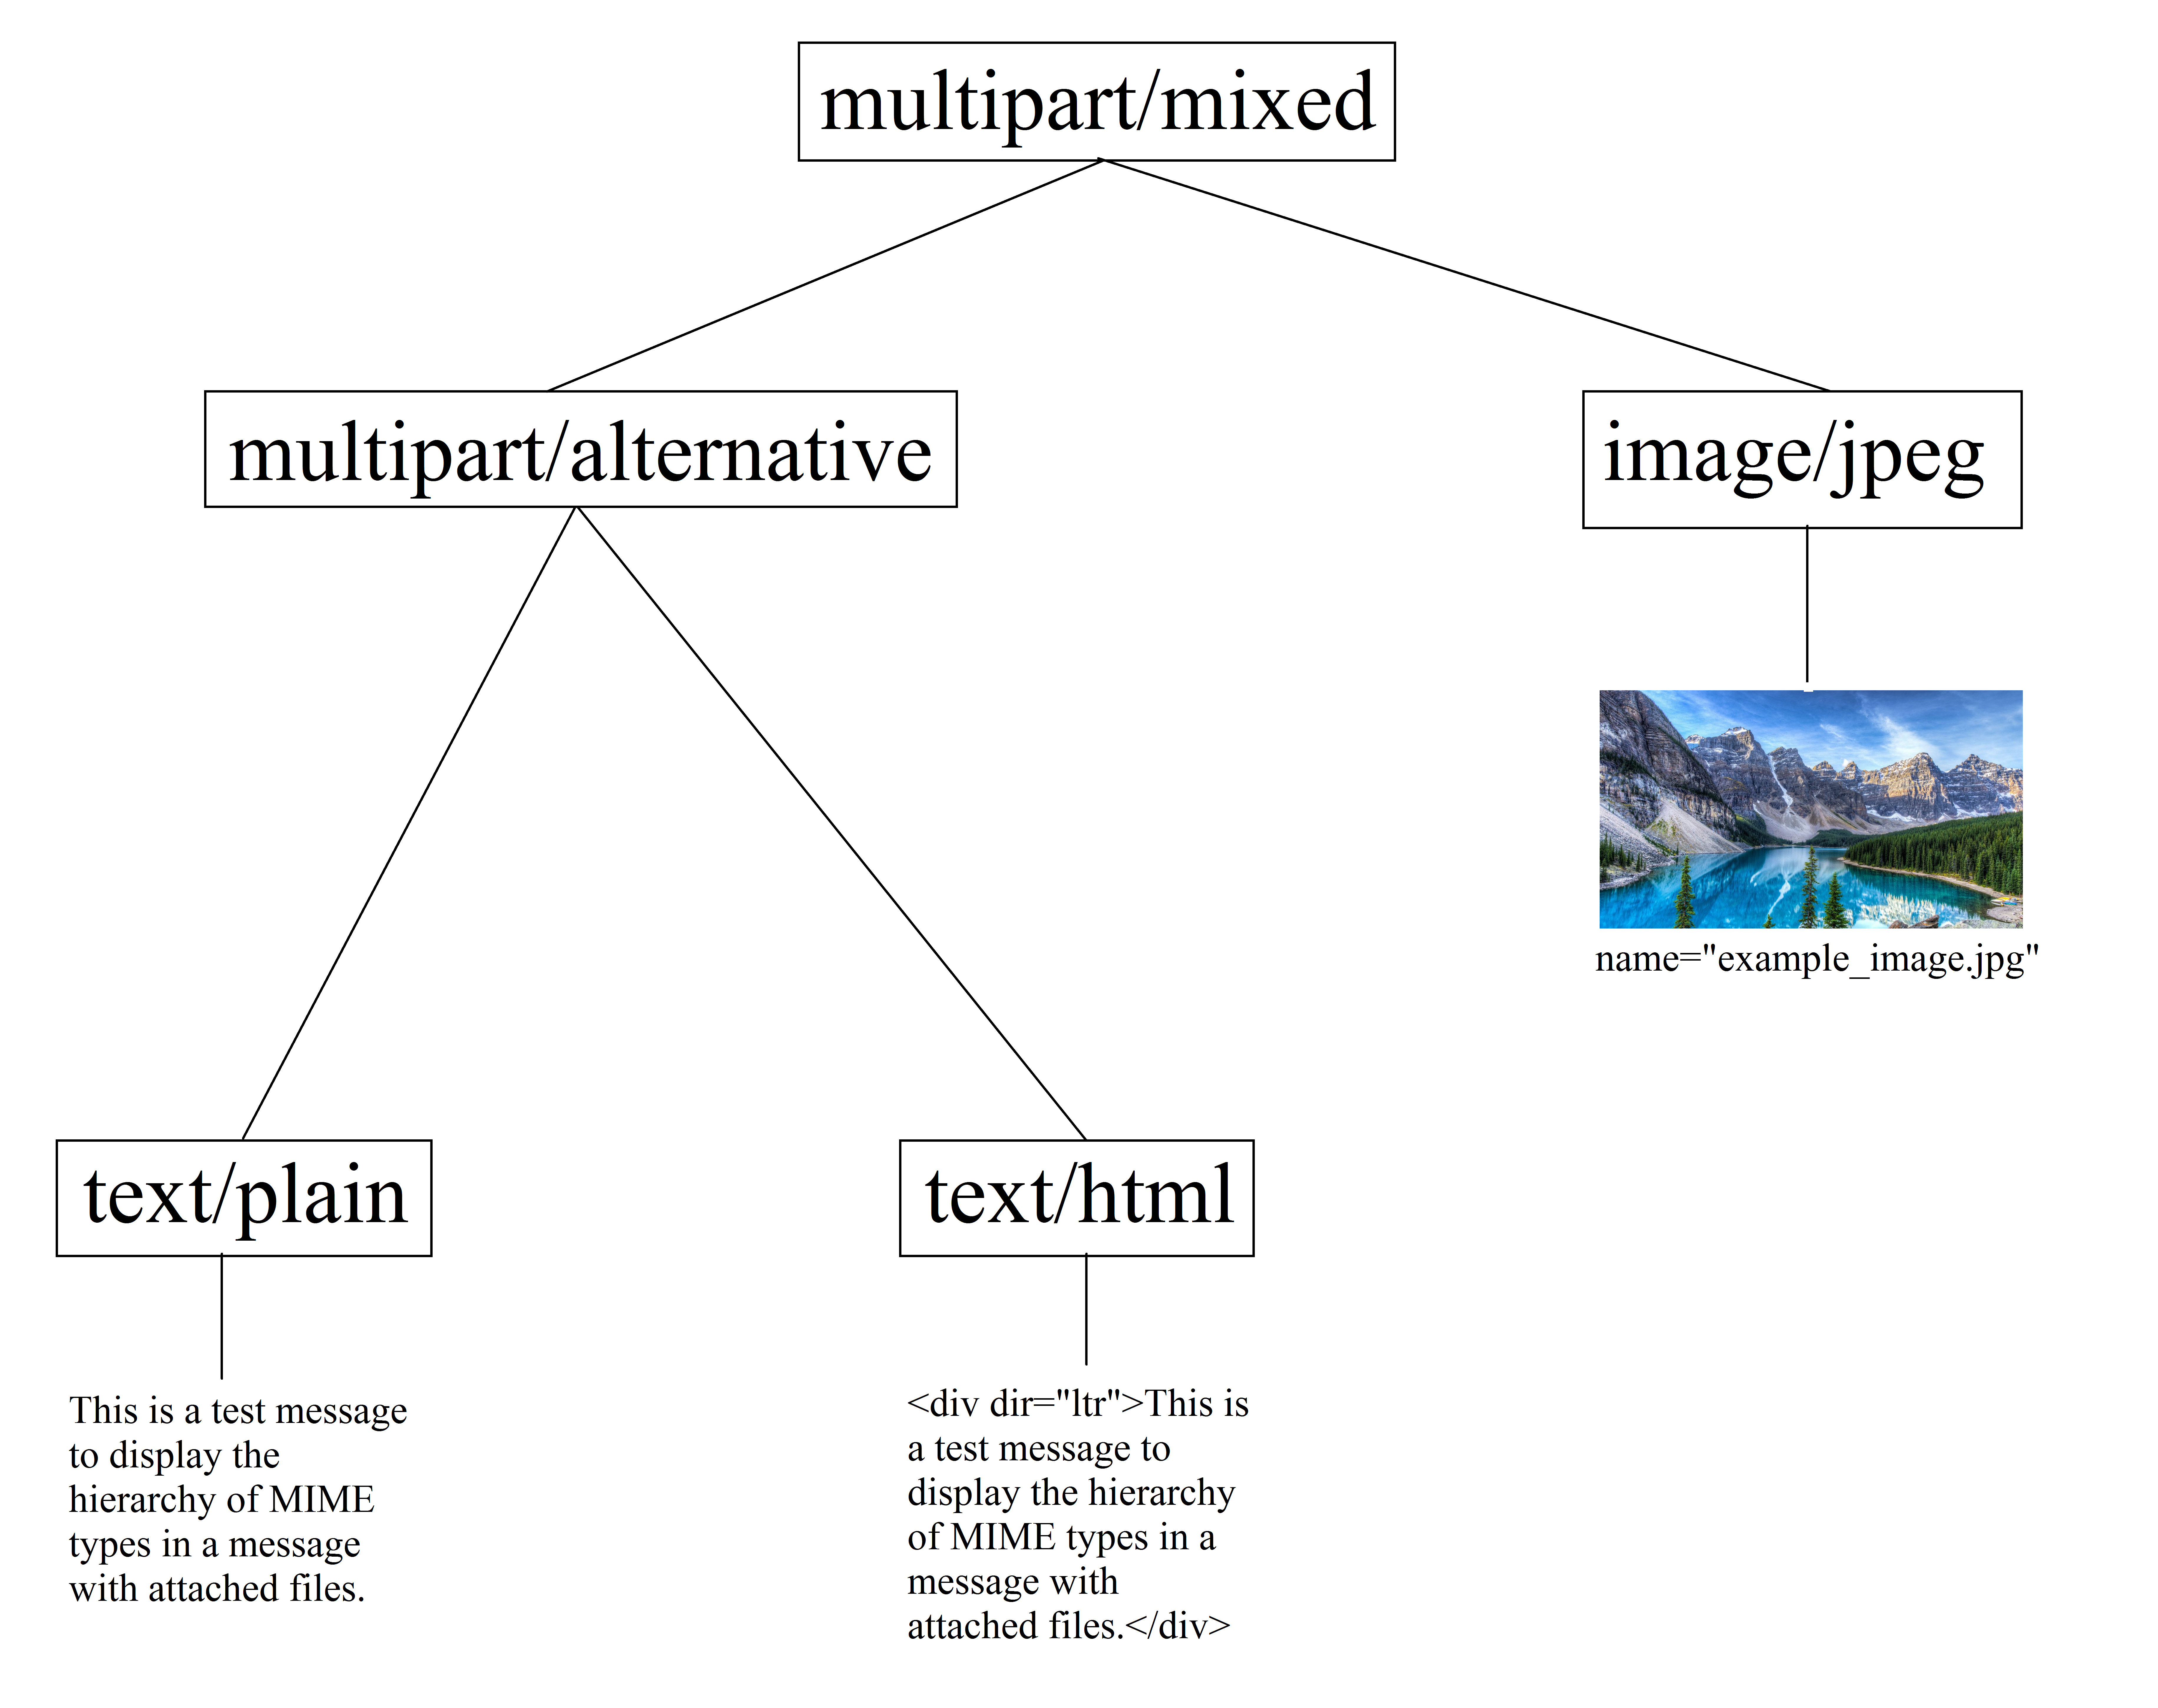
\includegraphics[width = 0.9\textwidth]{Imagenes/Bitmap/tree-content-type.png}}%
		\caption{Estructura arbórea de tipos MIME de un e-mail de ejemplo}%
		\label{fig:content-type}
		Imagen extraída de \cite{mitfg}
	\end{figure}

	\item\textit{Content-Disposition}: esta cabecera indica la forma de presentación de la parte del mensaje a la que pertenece. Puede tener dos posibles valores: \textit{inline} (que se utiliza cuando el contenido debe ser mostrado al mismo tiempo que el cuerpo del mensaje, como por ejemplo cuando se inserta una imagen en el texto y no como archivo adjunto) y \textit{attachment} (este valor determinará que la parte del mensaje requerirá algún tipo de acción por parte del usuario para visualizar el contenido, como por ejemplo en el caso de adjuntar un archivo). Además, esta cabecera dispone de distintos campos que reflejan más información acerca del contenido, como puede ser el nombre del archivo y la fecha de creación o de modificación. A continuación se presenta un ejemplo extraído de \cite{rfc2183} de esta cabecera y los campos que pueden acompañarle:
	
	\begin{lstlisting}
		Content-Disposition: attachment; filename=genome.jpeg;
		modification-date="Wed, 12 Feb 1997 16:29:51 -0500";
	\end{lstlisting}
	
	También puede observarse esta cabecera en la última parte del mensaje de ejemplo de la figura \ref{fig:examplemime}.
	
	\begin{figure}[t]
		\centering%
		\centerline{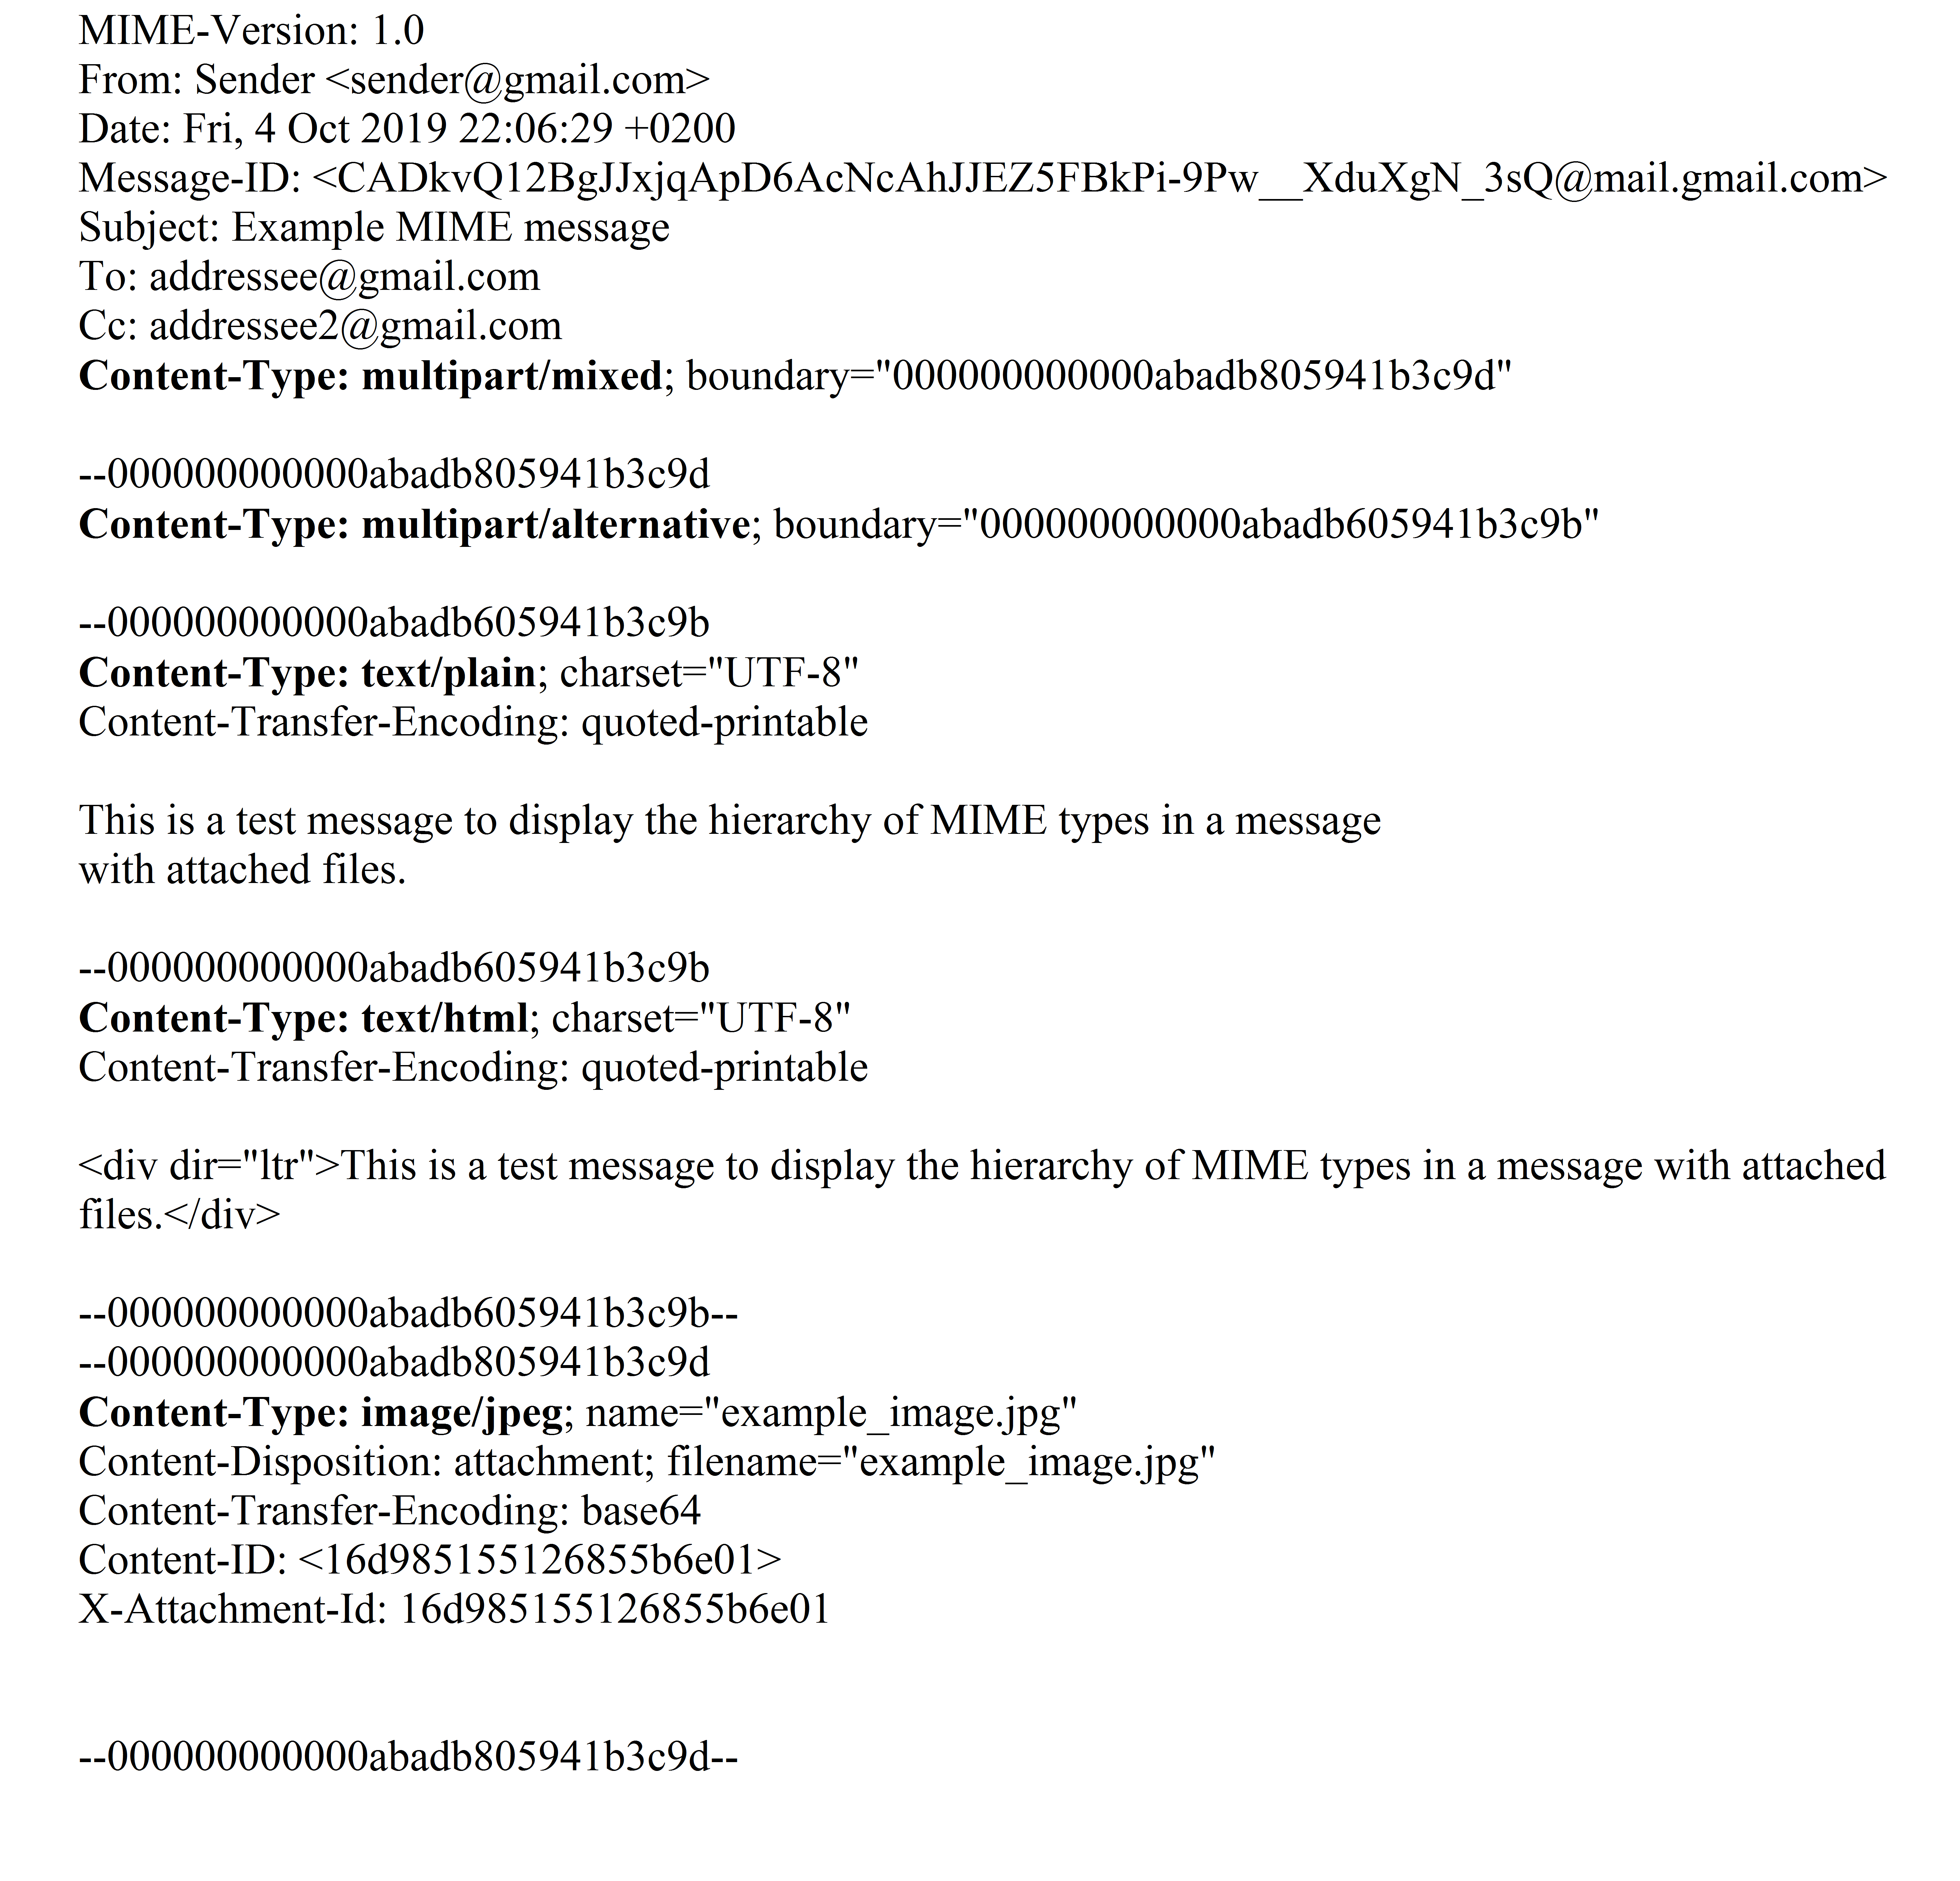
\includegraphics[width = 0.9\textwidth]{Imagenes/Bitmap/exampleMime.png}}%
		\caption{Mensaje MIME de la figura \ref{fig:content-type}}%
		\label{fig:examplemime}
		Imagen extraída de \cite{mitfg}
	\end{figure}
	\item\textit{Content-Transfer-Encoding}: cuando se mandan archivos en un correo electrónico, a veces estos se codifican como 8-bit o archivos binarios, codificaciones no soportadas por determinados protocolos. Por este motivo, es necesario poseer un estándar que especifique cómo debe re-codificarse este tipo de información en un formato 7-bit. La cabecera \textit{Content-Transfer-Encoding} \citep[Sección 5]{rfc1341} indica al cliente qué tipo de transformación se ha efectuado para que este sea capaz de recuperar los datos originales. Los posibles valores son \textit{base64} \citep{rfc4648, rfc2045}, \textit{quoted-printable} \citep{rfc1521}, \textit{8bit}, \textit{7bit}, \textit{binary} y \textit{x-token}. Todos ellos hacen referencia a un tipo de codificación que se encuentran fuera del alcance de este trabajo y para las que se recomienda consultar las referencias bibliográficas en caso de querer profundizar en ellas.
\end{itemize}

\subsection{SMTP}\label{ss:smtp}
El SMTP (cuyas siglas hacen referencia a \textit{Simple Mail Transfer Protocol}) es un protocolo de red orientado a conexión utilizado para el intercambio de correos electrónicos. Originalmente fue definido por \cite{rfc821} (para especificar cómo llevar a cabo el envío de mensajes) y \cite{rfc822} (que presenta el formato que deben tener los e-mails). Actualmente, se deben consultar los RFC desarrollados por \cite{rfc5321} y \cite{rfc5322} que, respectivamente, sustituyen a los dos originales.

Al ser un protocolo de transferencia de mensajes, posee algunas limitaciones a la hora de recibir e-mails en el servidor de destino. Por ello, esta tarea se delega a otros protocolos como el POP (véase la sección \ref{ss:pop}) e IMAP (véase la sección \ref{ss:imap}), mientras que el SMTP se encarga única y exclusivamente del envío.

Cuando se hace uso del SMTP un correo electrónico es enviado (esta acción de denota con la palabra \textit{push}) de un servidor a otro hasta que alcanza su destino. El mensaje se encamina en función del servidor de correo de destino, en lugar de hacerlo en función de los destinatarios individuales del mensaje especificados durante la conexión del cliente al servidor SMTP. Gracias a que este protocolo dispone de una función para iniciar el procesamiento de la cola de correo, un servidor de correo conectado de forma intermitente puede extraer mensajes de otro servidor remoto cuando sea necesario.

\subsection{POP}\label{ss:pop}
El POP (cuyas siglas hacen referencia a \textit{Post Office Protocol}) es un protocolo de aplicación en el modelo OSI utilizado para la obtención de e-mails almacenados en un servidor remoto de Internet denominado servidor POP. Originalmente fue definido por \cite{rfc918},que especificó la primera versión de POP, también conocida como POP1. La versión actual de POP, POP3 (en general cuando se habla de POP se refiere a esta versión), fue detallada por \cite{rfc1939}.

El protocolo POP posee numerosos comandos que hacen posible la conexión manual con el servidor POP3. Además, soporta otros como LIST, RETR y DELE, que permiten la gestión de los mensajes del usuario con acciones como mostrarlos, descargarlos o borrarlos, respectivamente.

POP3 fue diseñado para la tarea de recepción de correos electrónicos. Gracias a este protocolo, los usuarios con conexiones a Internet intermitentes o muy lentas pueden descargar sus mensajes mientras se encuentran conectados a la red y consultarlos estando \textit{offline}. La sucesión de operaciones más común se produce cuando un cliente se conecta, descarga todos sus mensajes, los almacena en su dispositivo local como e-mails nuevos, se borran del servidor y, por último, el usuario se desconecta. Sin embargo, algunos clientes de correo incluyen la opción de dejar los mensajes almacenados en el servidor en lugar de borrarlos. Estos utilizan el comando UIDL (\textit{Unique IDentification Listing}) el cual, a diferencia del resto de instrucciones de POP3, no identifica el correo electrónico a través del número ordinal asociado por el servidor, ya que generaría problemas si un cliente tratara de dejar ciertos mensajes en el servidor debido a que este número cambiaría de una conexión a otra. En lugar de ello, asigna a cada mensaje un identificador constituido por una cadena de caracteres única y permanente. De esta manera, se puede determinar fácilmente qué mensajes se quieren almacenar en el servidor a la vez que se descargan.

Al igual que otros protocolos más antiguos, POP3 utiliza un mecanismo de firma sin encriptación. De hecho, la transmisión de contraseñas POP3 en texto plano continúa ocurriendo. Hoy en día, POP3 tiene varios métodos de autenticación que ofrecen un amplio rango de niveles de protección contra accesos ilegales a las bandejas de correo de los usuarios.

La ventaja de POP3 frente a otros protocolos es que entre el cliente y el servidor no es necesario mandar un gran número de comandos para comunicarse. Este protocolo también resulta muy útil cuando no se cuenta con una conexión constante a Internet o a la red que aloja al servidor.

\subsection{IMAP}\label{ss:imap}
El IMAP (cuyas siglas hacen referencia a \textit{Internet Message Access Protocol}) es un protocolo de aplicación diseñado como alternativa al POP (véase la sección \ref{ss:pop}) en 1986, el cual permite el acceso a los mensajes almacenados en un servidor de Internet. Al igual que con el POP, con el IMAP es posible acceder a la cuenta de correo electrónico desde cualquier dispositivo con conexión a Internet. La versión actual del IMAP (IMAP versión 4 revisión 1 o IMAP4rev1) fue definida por \cite{rfc3501}.

A diferencia del POP, el IMAP abre la puerta a la gestión de la misma bandeja de entrada por parte de múltiples clientes. Esta característica se produce gracias a las principales diferencias entre los dos protocolos: el IMAP no elimina los mensajes del servidor hasta que el cliente lo solicite explícitamente (mientras que el POP los borra por defecto, lo que hace imposible acceder a ellos desde otro dispositivo que no haya descargado previamente los correos electrónicos) y tampoco descarga los e-mails en el dispositivo del usuario, aunque opcionalmente es factible tener una copia local de los mismos. Esta última propiedad del IMAP da lugar a algunas ventajas frente al POP. Una de ellas es la posibilidad e notificar de manera inmediata de la llegada de un nuevo correo electrónico (ya que el IMAP funciona con una conexión cliente-servidor permanente), mientras que el POP verifica si hay nuevos mensajes cada pocos minutos (lo cual provoca un aumento apreciable del tráfico y del tiempo que el usuario tiene que esperar para enviar una solicitud al servidor, ya que es necesario completar primero la descarga de todos los mensajes nuevos). Por otro lado, gracias al IMAP, los usuarios pueden crear carpetas compartidas con otras personas (esta funcionalidad depende del servidor de correo) y los e-mails no ocupan espacio de memoria en el dispositivo local, mientras que el POP los descarga independientemente de si van a ser leídos o no (estrictamente hablando, el IMAP tiene que descargar el mensaje cuando va a ser leído, pero se trata de archivos temporales y solo se extraen las cabeceras de los correos electrónicos a la hora de gestionar la bandeja de entrada). Precisamente, el hecho de evitar la descarga del e-mail, permite al usuario gestoinar carpetas, plantillas y borradores en el servidor además de poder llevar a cabo una búsqueda en la bandeja de entrada mediante palabras clave.